\subsection{Digitale Transformation mit Internet of Things}

Eine Umsetzung von Industrie-4.0-Lösungen setzt technische, organisatorische und normative Bedingungen voraus. Während einige Anforderungen für alle Bereiche in der Industrie gelten, unterscheiden sich explizite Anforderungen und Lösungen je nach individuellen Ausgangssituationen von Branchen und Unternehmen \citep{Bauer2014}. Dieses Kapitel soll einen mehrdimensionalen Einstieg in die Thematik digitale Transformation bringen. Zuerst wird ein Branchenbezug für die Energiewirtschaft hergestellt. Anschließend folgen allgemeine Herausforderungen zur Umsetzung von IoT-Lösungen für die digitale Transformation. Daraufhin wird eine Referenzarchitektur zur Bewältigung dieser Herausforderungen vorgestellt. Einen wesentlichen Stellenwert in Transformationsprozessen hat das Cloud Computing als technische Voraussetzung, sodass es einer detaillierteren Erläuterung als in \ref{technologien} bedarf. 

\subsubsection{Der Wandel im Energiesektor} \label{energy}

Der Wandel in der gesamten Industrielandschaft von der Mechanisierung und Automatisierung zur Digitalisierung betrifft auf ähnliche Weise auch den Energiesektor. Es gibt in Deutschland kaum eine Branche, die sich innerhalb von zwanzig Jahren so rasant geändert hat wie die Energiewirtschaft \citep{Doleski2015}. Treiber dieser schnellen Entwicklungen sind in erster Linie politisch"=regulatorische Faktoren, welche für darauffolgende Anforderungen die Parameter darstellen.
\\Bis 1998 unterlag die Energieproduktion in Deutschland monopolistischen Strukturen. Einige wenige Versorgungsunternehmen produzierten in zentralen Werken wie Kernkraftanlagen oder Kohlekraftwerke und schleusten die gewonnene Energie in die Netze ein \citep{Utecht2018}. Die Konsumenten hatten bei der Auswahl ihres Energielieferanten kaum Entscheidungsfreiheit. Mit der Liberalisierung und Privatisierung der Strommärkte öffnete sich jedoch der Binnenmarkt für den Wettbewerb \citep{Doleski2017}. Vor allem durch das \textit{Unbundling}, also der Trennung von Erzeugung und Vertrieb, betraten mehrere Dienstleister für unterstützende Tätigkeiten den Markt. Auch in der Produktion stieg wegen des Wegfalls von Gebietsmonopolen der Trend von zentralen Produktionswerken zu lokalen Erzeugern in der Nähe des Verbrauchers an \citep{Utecht2018}. Grundlegende Veränderungen und Innovationen kamen mit dem Ausbau von erneuerbaren Energiequellen nach der Verabschiedung des Erneuerbare-Energien-Gesetzes von 2000 zur systematischen Förderung von regenerativen Energiequellen. Vor allem nach der Nuklearkatastrophe 2011 in Fukushima wurde die Energiewende stark beschleunigt \citep{Doleski2015}. Der geplante Ausstieg aus Atomkraft und Kohle zwang die Branchen, sich strukturell in der Wertschöpfungskette zu verändern. Die Herausforderung bestand vor allem darin, innerhalb der strengen gesetzlichen Regularien und eines angespannten Finanzrahmens neue Geschäftsfelder zu erschließen \citep{Doleski2015}. So veränderte sich der Produktionstrend von zentraler Erzeugung zu dezentraler Erzeugung mit z.B. Windkraft und Photovoltaik. Die neuen Produktionsmechanismen bedeuten technisch gesehen einen enormen Anstieg der Steuerungskomplexität und eine Belastung der Netzinfrastruktur. Während die Produktion nun vielmehr von schwankenden Umweltbedingungen abhängig ist, bleiben die Anforderungen im Verbrauch wie die ständige Verfügbarkeit oder die stabile 50-Hz-Netzfrequenz unverändert \citep{Utecht2018}.
\\\\
\noindent Es sind zwar politisch-regulatorische und ökologische Faktoren, die Umwälzungen in der Energiewirtschaft erzwingen, aber die dezentrale und fluktuierende Energieerzeugung erfordert digitale Lösungen \citep{Doleski2017}. Der Digitalisierung wird eine Schlüsselrolle bei der Lösungsfindung für Dezentralisierung, Flexibilisierung sowie für die effiziente Nutzung von Ressourcen und Energie zugewiesen \citep{FraunhoferISE}. Als \textit{Enabler} für die Energiewende konvergiert die IT-Branche immer mehr mit energiewirtschaftlicher Leistungserstellung \citep{Doleski2015}. Laut dem \citet{BWE2015} wird die Energiebranche eine der ersten voll digitalisierten Branchen der deutschen Volkswirtschaft sein. Zwar kann der Strom nicht digitalisiert werden, aber die Vielzahl von technischen Komponenten in Anlagen müssen sowohl untereinander als auch mit dem Menschen kommunizieren können. Anders als früher ist das gesamte Stromnetz abhängig von einer Vielzahl von Erzeugungsanlagen, die ihren Strom nun in ein intelligentes Stromnetz (Smart Grid) einschleusen müssen. Das Smart Grid kombiniert in einem Netz die Erzeugung, Speicherung und den Verbrauch der Energie. Die dezentralen Erzeugungen werden durch eine zentrale Steuerung aufeinandender abgestimmt, sodass die Leistungsschwankungen ausgeglichen werden können \citep{Krone2017}. Die Intelligenz wird durch den Datentransport von der Erzeugungsanlage in das Netz gewährleistet. Wenn es zu viele unkoordinierte Anlagen gibt, die ihre Produktionsmengen und ihren Zustand nicht kommunizieren können, kann es zu Instabilität im Netz führen \citep{Umweltbundesamt2018}. Damit die einzelnen Anlagen miteinander kommunizieren können, müssen sie Teil eines \ac{iot}-Netzwerks sein. Somit können sie ihre Umgebungs- und Zustandsdaten eigenständig an ein \acf{cms} senden, das die Daten z.B. in der Cloud sammelt. Für die dort erstellten digitalen Zwillinge der realen Anlagen können auf Grundlage von Analysen der vergangenen und aktuellen Daten prädiktive Wartungsmaßnahmen abgeleitet werden. Daraus kann eine Verbesserung der Qualität und eine höhere Verfügbarkeit des Dienstes resultieren \citep{Utecht2018}.

\begin{figure}[h]
  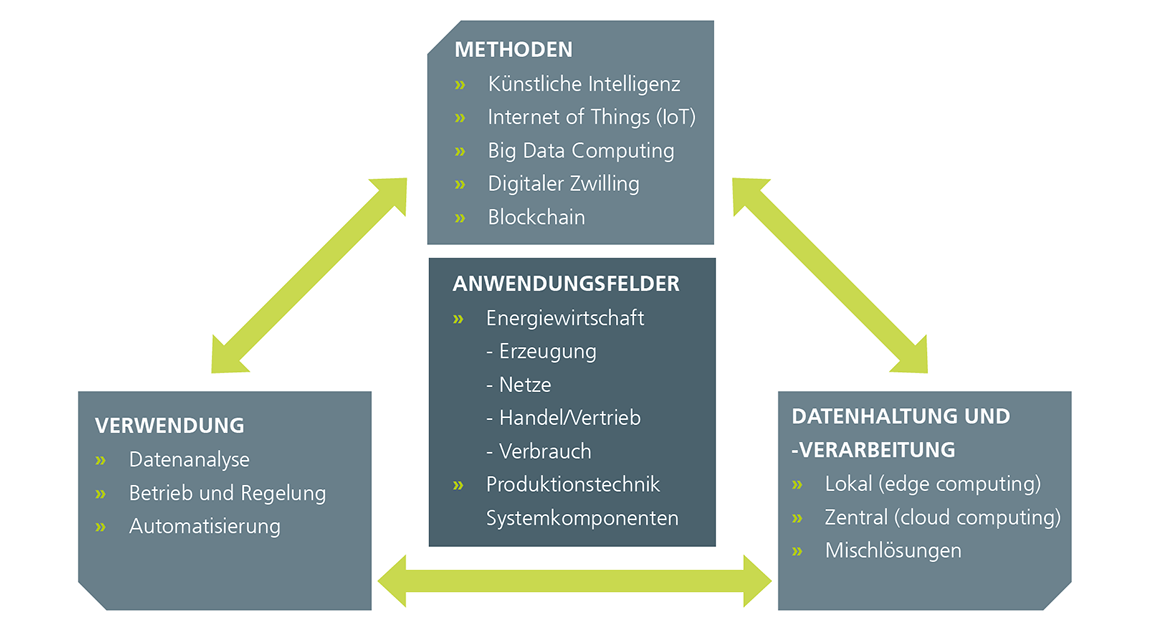
\includegraphics[width=1.0\linewidth]{dimensionen_digitalisierung_fraunhofer.png}
  \caption[Dimensionen der Digitalisierung]{Dimensionen der Digitalisierung \citep{FraunhoferISE}}
  \label{dimensionen}
\end{figure}

\noindent Die rasanten Entwicklungen in den letzten 20 Jahren zeigen, wie schnell sich die Branche verändern kann. Um in Zukunft auf dem Markt zu überleben, müssen sich Energieproduzenten und Diensteister in einem ständigen Anpassungsprozess befinden \citep{Doleski2015}. Essenziell für eine Anpassung an die fortwährende Vernetzung der Produktionswelt ist der Aufbau und die Umsetzung einer unternehmensspezifischen Digitalisierungsstrategie \citep{Koester2017}. Die Herausforderung besteht vor allem darin, die verschiedenen Disziplinen und Dimensionen in der digitalisierten Welt zu berücksichtigen (s. Abbildung \ref{dimensionen}).  Da die Energiebranche besonders gesellschaftlich eine wichtige Rolle innehat, sind die Themen Datenschutz und Sicherheit nicht zu vernachlässigen \citep{Utecht2018}.


\subsubsection{Die Herausforderung IoT}\label{general}

Im Rahmen der Industrie 4.0, die eine Spezialisierung des Internet der Dinge und Dienste darstellt, wachsen die virtuelle und reale Welt zusammen. Daraus ergibt sich die Herausforderung, die Anforderungen der IT, der Elektrotechnik sowie des Maschinenbaus miteinander zu vereinen \citep{Huebner2017}.

\noindent Aufgrund der heterogenen Landschaften und Aussgangssituationen der Unternehmen sei eine Standardisierung der Technologien laut \citet{Bauer2014} unerlässlich. Des weiteren ist die Weiterentwicklung von Breitbandnetzwerken für eine echtzeitfähige Kommunikation von Systemen eine Grundvoraussetzung. Notwendig sind außerdem qualitätsgesicherte Dienste im Internet, die robust gegen Störungen sind. Der Begriff \textit{Internet der Dinge und Dienste} bezieht auf vernetzte Komponenten wie physische Systeme, aber auch auf virtuelle Anwendungen. Da sich die Anzahl und die Beschaffenheit der Applikationen ebenso rasant ändern kann wie die der Geräte, sind eine standardisierte Laufzeitumgebung und Kommunikation für diese von großer Bedeutung. Nicht zu vernachlässigen sind dabei die Sicherheitsaspekte. Die \ac{iot}-Anwendungen bilden eine große Angriffsfläche für Hacker, die durch Sabotage und Manipulation der Systeme eine große Gefahr dartellen. Ein historisches Beispiel für solch eine Gefahr sind die Stuxnet-Angriffe von 2010 auf iranische Atomfabriken \citep{Bauer2014}.

\noindent Allgemein können die Anforderungen und Voraussetzungen für eine \ac{iot}-Lösung auf folgende Begriffe projiziert werden \citep{Acharya2019}:

\begin{itemize}
  \item Skalierbarkeit und Flexibilität
  \item Schnelligkeit
  \item (Ausfall-)Sicherheit
  \item Qualität
\end{itemize}

\subsubsection{Referenzarchitektur}\label{rami}

Für die Bewältigung der oben aufgeführten Herausforderungen veröffentlichte die Plattform Industrie 4.0 das \glqq Referenzarchitekturmodell Industrie 4.0\grqq{} (RAMI 4.0) sowie das Konzept zur \glqq Industrie-4.0-Komponente\grqq{}. Beide Modelle wurden 2016 nach DIN SPEC 91345 der Standardisierung zugeführt \citep{Beuth2016}.

\paragraph{RAMI 4.0} ist ein branchenübergreifendes Rahmenwerk, in dem Aufgaben und Abläufe der gesamten Wertschöpfung in überschaubare Teile zerlegt und entsprechenden Normen und Standards zugeordnet werden. Das dreidimensionale Modell ist in Anlehnung auf das Smart Grid Modell erstellt und kapselt die wichtigsten Funktionalitäten aus den verschiedenen Disziplinen in Schichten. Dies schafft Flexibilität für die Konzeptionisierung und Realisierung von Industrie-4.0-Lösungen \citep{Huebner2017}.
\\
Für die Migration von Produktionsgegenständen von der heutigen in die Industrie"=4.0"=Welt soll der gesamte Produktlebenszyklus in Daten erfasst und IT"=seitig einheitlich und durchgängig abgebildet werden. Die senkrechte Achse behandelt die IT"=Sicht, die die vertikale Integration der Assets in die Geschäftslogik und deren echtzeitfähige Vernetzung im Produktionsprozess beschreibt. Zu den Assets werden sowohl alle in der Anlage verbauten physischen Komponenten als auch andere Vermögensgegenstände wie Software oder Patente, aber auch Menschen, gezählt \citep{Adolphs2017}. Mit der Ergänzung des Assets um eine \textit{Verwaltungsschale} entsteht die \textit{Industrie-4.0-Komponente}. Die Verwaltungsschale ist das Bindeglied zwischen der realen und der virtuellen Welt. Mit dessen Hilfe wird ein virtuelles Abbild des Assets samt der dazugehörigen Funktionen und Daten erzeugt. Die IT-technische Beschreibung ermöglicht die eindeutige Identifizierung des Assets z.B. durch die \ac{uri}-Adresse im gesamten Wertschöpfungsprozess. Die Aktivitäten für den Übergang in die virtuelle Welt sind in der Integrationsschicht enthalten. Die Dienste zur Steuerung der Integration werden von der Kommunikationsschicht bereitgestellt. Sie dient außerdem der Vereinheitlichung der Kommunikation mit einem einheitlichen Datenformat \citep{BITKOM2015}. Für die Datenkommunikation wird der Standard für industrielle Kommunikation \ac{opcua} empfohlen. Ursache dafür ist zum einen die plattformunabhängige, \ac{soa} und zum anderen die Fähigkeit, die Maschine"=zu"=Maschine"=Kommunikation semantisch zu beschreiben.
\begin{figure}[h]
  \centering
  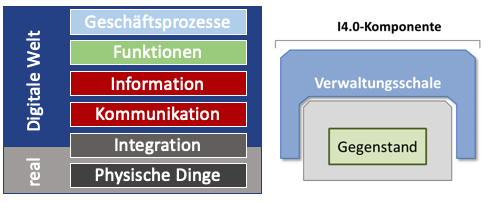
\includegraphics[width=0.7\linewidth]{IT_Sicht.png}
  \caption[IT-sicht und Industrie-4.0-Komponente]{IT-sicht und Industrie-4.0-Komponente (in Anlehnung an \citet[S. 118]{Adolphs2017}) }
  \label{it_layer}
\end{figure}
Anschließend werden die übertragenen Daten in der Informationsschicht gehalten, wo sie in einer Laufzeitumgebung in einen Regelkontext gebracht werden. Hier werden Regeln für Ereignisse und den Zugriff auf Daten definiert, die in der Funktionsschicht verarbeitet werden. Die tatsächlichen Funktionen eines Assets werden in der Funktionsschicht formal beschrieben. In der funktionalen Schicht befinden sich die Daten in einer Laufzeit- und Modellierungsumgebung für Dienste, die unter anderem Geschäftsprozesse unterstützen. Mit dieser Plattform können die Funktionen horizontal in die Wertschöpfung integriert werden \citep{Huebner2017}. Zusätzlich kann in der Funktionssicht auf ERP-Funktionen zugegriffen werden. Diese entstehen in der Geschäftssicht, in der die Modellierung der Regeln für die Geschäftsprozessabwicklung stattfindet. Letztendlich werden die Assets und deren Funktionen hier in die Organisation und Geschäftsprozesse integriert.
\\\\
Jede dieser IT-Schichten liegt an zwei wagerechten Achsen an, welche die horizontale Integration der Produktionsgegenstände in den gesamten Produktionprozess beschreiben. Die linke Achse soll den gesamten Lebenszyklus von Assets abbilden, während die rechte Achse diese in Hierarchiestufen der Produktions- und Automatisierungstechnik anordnet. Somit können externe Akteure wie Lieferanten oder Kunden, aber auch das erzeugte Produkt in das Industrie-4.0-Netzwerk aufgenommen werden \citep{BITKOM2015}.


% ************* CLOUD COMPUTING ******************
\subsubsection{Das neue Paradigma: Cloud Computing} \label{cloud}

Flexibilität, Skalierbarkeit, Schnelligkeit, Sicherheit und Qualität präsentieren sich als die wichtigsten Voraussetzungen für die erfolgreiche digitale Transformation eines Unternehmens \citep{Acharya2019}. Für die Erzielung dieser Ziele spielt die in \ref{technologien} bereits kurz erläuterte Cloud eine Schlüsselrolle. Denn die Technologien in der Industrie 4.0 sind zwar nicht neu, aber sie müssen in verschiedenen Kombinationen bei niedrigen Preisen und unabhängig vom Ort stets verfügbar sein. Bei alledem wird dem Nutzer je nach Bedarf das Errichten von IT-Infrastruktur und IT-Ressourcen von dem Cloud-Dienstleister abgenommen \citep{Dzombeta2017}. Entsprechend können die Cloud-Dienste aus folgenden Varianten nach nutzungsbasierten Abrechnungsmodellen wie z.B. dem Pay-Per-Use-Prinzip erworben werden:

\paragraph{\ac{iaas}} Bei dieser Variante stellt das Dienstleistungsunternehmen die notwendige Hardware in virtueller Form zur Verfügung. Es können je nach benötigter Menge Speicherplatz, Prozessorleistung oder Netzkapazitäten bestellt oder wieder abbestellt werden \citep{Dzombeta2017}. Kostentechnisch bietet das einen großen Vorteil, da die Server von den Anbietern angeschafft, betrieben und gewartet werden, sodass nur die verbrauchte oder vereinbarte Kapazität in Rechnung gestellt wird. Zu den global dominierenden Anbietern gehören Amazon, Microsoft und Google, die in Nordamerika, Europa und Ostasien eine hohe Dichte an Rechenzentren aufweisen \citep{Acharya2019}.

\paragraph{\ac{paas}} Das Dienstleistungsangebot dieser Variante beläuft sich auf die Bereitstellung von Middleware, Laufzeit- und Entwicklungsumgebungen zur Erstellung von Anwendungen, Datenbanken und Webservices. Über definierte Schnittstellen (APIs) kann auf die Entwicklungsumgebung zugegriffen werden \citep{Dzombeta2017}. Da die Plattform auf \ac{iaas} basiert, fällt die Administration von Servern weg \citep{Acharya2019}.

\paragraph{\ac{saas}} Kunden können bei dieser Form meist über Webbrowser auf Software(-pakete) zugreifen, die auf der Infrastuktur des Anbieters gehostet sind. Dabei übernimmt der Anbieter Aufgaben wie Installation, Wartung und Aktualisierung der Software \citep{Utecht2018}. Dieses Prinzip ermöglicht einen schnellen Einsatz sowie eine einfache Austauschbarkeit der Software bei niedrigen Kosten. Aufgrund der Unabhängigkeit von lokalen Installationen kann die Software ortsunabhängig bei verfügbarer Internetverbindung genutzt werden \citep{Dzombeta2017}.

\vspace{0.5cm}
\noindent Die verschiedenen Modelle können auch in Kombination mit dem On-Premise-System genutzt werden.

\noindent Mit diesen Modellen bietet die Cloud einen Raum für die verschiedenen Teilsysteme, die im Industrie"=4.0"=Netzwerk miteinander kommunizieren und Dienste anbieten. Eine \acf{soa} ermöglicht die Interoperabilität der Akteure wie Komponentenhersteller, Automatisierer, Maschinenbauer und Softwarefirmen ohne Master"=Slave"=Beziehungen. In der \ac{soa}-Welt wird nicht mehr zwischen Hard- und Software unterschieden, sodass maschinelle Komponenten ihre Daten genau so als Service zur Verfügung stellen können wie eine Software ihre Funktionen bereitstellt \citep{Adolphs2017}. Entwicklungen wie diese verändern die grundsätzliche Denkweise in der Softwareentwicklung. Alte Architekturen werden von neuen Architekturen wie die \textit{Microservice-Architektur} vertrieben \citep{Acharya2019}.

\begin{figure}[h]
  \centering
  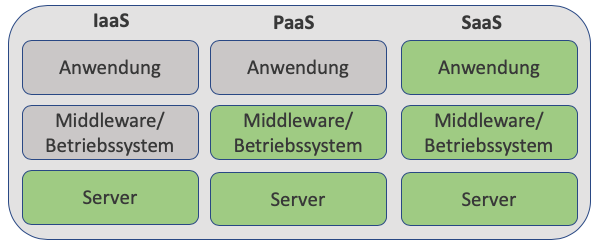
\includegraphics[width=0.8\linewidth]{cloud_variant.png}
  \caption[Die Cloud-Service-Modelle]{Die Cloud-Service-Modelle (In Anlehnung an \citet[S. 88]{Utecht2018})}
  \label{}
\end{figure}

\paragraph{Cloud-native Anwendungen und Microservices}

Die Eigenschaft cloud-nativ besitzen jene Anwendungen, welche in der Cloud \glqq geboren\grqq{} sind und durch Auschöpfung des Cloud"=Potenzials die Flexibilität, Agilität und Skalierbarkeit von Cloud-Lösungen unterstützen \citep{Acharya2019}. Besonders ist dabei der agile und schnelle Entwicklungsprozess der Software. Eine cloud"=native Anwendung besteht aus mehreren isolierten Services, die unabhängig voneinander entwickelt werden können. Konventionelle Anwendungen sind im Gegensatz dazu monolithischer Natur und basieren meist auf der 3"=Tier"=Architektur. Mit den Bestandteilen Benutzeroberfläche, Datenbank und Anwendungsserver bilden sie ein geschlossenes System. Kleinste Änderungen an einem der Bestandteile führen zu aufwendigen Maßnahmen zur Anpassung des Gesamtsystems \citep{Utecht2018}.
Anders als monolithische Architekturen zeichnet sich die Microservice-Architektur durch ihre einfache und schnelle Erweiterbarkeit und Anpassungsfähigkeit aus. Ein Microservice ist eine spezielle Funktion, oft Geschäftsfunktion, welche in Containern in in einer isolierten Umgebung ausgeliefert wird und meist an eine eigene Datenbank angebunden ist. In einer Anwendung kommunizieren diese Microservices über APIs oder Messaging"=Prokolle miteinander und bilden ein Gesamtsystem mit heterogenen Datenquellen. Sollte eine Funktion ein Update erforden, muss lediglich der Microservice  gewartet werden. Wenn das System eine neue Funktion erfordert, kann ein neuer Microservice einfach hinzugefügt werden, ohne Abhängigkeiten im Gesamtsystem zu stören. Infrastrukturressourcen können bei Bedarf dynamisch zu- oder abgewiesen werden \citep{Acharya2019}.


